\documentclass[slidetop,mathserif,red]{beamer}

\usepackage[utf8]{inputenc}
\usepackage[T1]{fontenc}
\newcommand{\specs}{\mathcal{SP}} % satisfaction relation for specifications
\usepackage{amsmath}
\usepackage[british]{babel}
\usepackage{graphicx}
\usepackage{lmodern}
\usepackage{url}
\usepackage{verbatim}
\usepackage[all]{xy}
\usepackage{listings}
\usepackage{smartdiagram}
\usepackage{fancybox}
\usepackage{animate}

\usesmartdiagramlibrary{additions}

\definecolor{dgreen}{rgb}{0.0,0.47,0.0}
\definecolor{maroon}{rgb}{0.8,0.5,0.4}

\usepackage{xcolor}
\usepackage{colortbl}

\usetheme{Singapore}
\usecolortheme{lily}
\usepackage{etoolbox,refcount}
	
\graphicspath{{images/}}

\title{Research Ethics in relation to AI-assisted Adaptive Technology for mental health treatment}

\author[mukhiya]{{Suresh Kumar Mukhiya}}

\institute[Bergen University College]{ Western Norway University of Applied Sciences}

\date[Autumn 2017]{PCS 902 \\ Spring 2019\\ Bergen, Norway}

\subject{Research Ethics\\ www.skmukhiya.com.np}

\logo{\includegraphics[height=.05\textwidth]{hvl_logo_engelsk}}
\addtobeamertemplate{navigation symbols}{}{%
    \usebeamerfont{footline}%
    \usebeamercolor[fg]{footline}%
    \hspace{1em}%
    \insertframenumber/\inserttotalframenumber
}
\setbeamercolor{footline}{fg=blue}
\setbeamerfont{footline}{series=\bfseries}

\begin{document}


\begin{frame}
  \titlepage
\end{frame}

\begin{frame}{scientific oath}
  \textit{I acknowledge that I am a part of an international community of researchers. I will practise my activities in line with the \textbf{recognised standards} for good research practice. I shall conduct my research in an \textbf{honest} and \textbf{truthful} way and show respect for humans, animals, and nature. I shall use my knowledge and skills to the best of my \textbf{judgement} for the good of humanity and \textbf{for sustainable development}. I shall \textbf{not allow interests based on ideology, religion, ethnicity, prejudice, or material advantages} to overshadow my ethical responsibility as a researcher. }
\end{frame}

\section{Ph.D Project}

\begin{frame}{What am I doing?}
\begin{center}
	\includegraphics<1>[scale=0.19]{project1}
\end{center}
\end{frame}

\begin{frame}{Use ICT technology for treatment of mental health problems}
\begin{center}
	\includegraphics<1>[width=\textwidth]{project2}
\end{center}
\end{frame}

%%%%%%%%%%%%%%%%%%%%%%%%%%%%%%%%%%%%%%%%%%%%%%%%%%%%%%%%%%%%%%%%%%%%%%%%%%%%%%%%%%%%%%%%%%%%%%%%%%%

\section{Backgrounds}
\begin{frame}{Machine Learning Approach}
    \begin{figure}[t]
\resizebox {\columnwidth} {!} {

\tikzset{every picture/.style={line width=0.75pt}} %set default line width to 0.75pt        

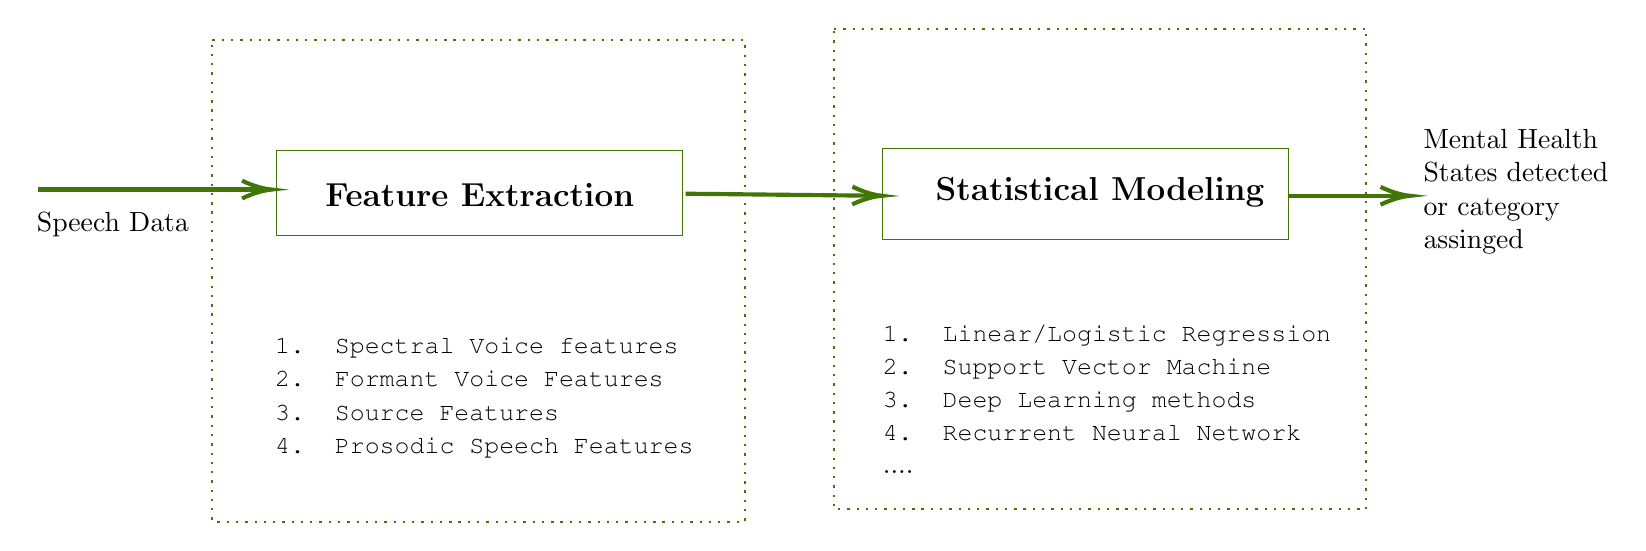
\begin{tikzpicture}[x=0.75pt,y=0.75pt,yscale=-1,xscale=1]
%uncomment if require: \path (0,247); %set diagram left start at 0, and has height of 247

%Shape: Rectangle [id:dp32459351977703954] 
\draw  [color={rgb, 255:red, 65; green, 117; blue, 5 }  ,draw opacity=1 ] (134,60) -- (329.5,60) -- (329.5,101) -- (134,101) -- cycle ;
%Shape: Rectangle [id:dp008190558981483909] 
\draw  [color={rgb, 255:red, 65; green, 117; blue, 5 }  ,draw opacity=1 ] (426,59) -- (621.5,59) -- (621.5,103) -- (426,103) -- cycle ;
%Shape: Rectangle [id:dp4086461697969652] 
\draw  [color={rgb, 255:red, 65; green, 117; blue, 5 }  ,draw opacity=1 ][dash pattern={on 0.84pt off 2.51pt}][line width=0.75]  (103,7) -- (359.5,7) -- (359.5,239) -- (103,239) -- cycle ;
%Shape: Rectangle [id:dp9009435343902048] 
\draw  [color={rgb, 255:red, 65; green, 117; blue, 5 }  ,draw opacity=1 ][dash pattern={on 0.84pt off 2.51pt}][line width=0.75]  (402.5,1.5) -- (659,1.5) -- (659,233) -- (402.5,233) -- cycle ;
%Straight Lines [id:da3400754300954796] 
\draw [color={rgb, 255:red, 65; green, 117; blue, 5 }  ,draw opacity=1 ][line width=1.5]    (19,79) -- (128.5,79) ;
\draw [shift={(131.5,79)}, rotate = 180] [color={rgb, 255:red, 65; green, 117; blue, 5 }  ,draw opacity=1 ][line width=1.5]    (14.21,-4.28) .. controls (9.04,-1.82) and (4.3,-0.39) .. (0,0) .. controls (4.3,0.39) and (9.04,1.82) .. (14.21,4.28)   ;

%Straight Lines [id:da8761870943412116] 
\draw [color={rgb, 255:red, 65; green, 117; blue, 5 }  ,draw opacity=1 ][line width=1.5]    (331,81) -- (422.5,81.97) ;
\draw [shift={(425.5,82)}, rotate = 180.61] [color={rgb, 255:red, 65; green, 117; blue, 5 }  ,draw opacity=1 ][line width=1.5]    (14.21,-4.28) .. controls (9.04,-1.82) and (4.3,-0.39) .. (0,0) .. controls (4.3,0.39) and (9.04,1.82) .. (14.21,4.28)   ;

%Straight Lines [id:da7294368618848919] 
\draw [color={rgb, 255:red, 65; green, 117; blue, 5 }  ,draw opacity=1 ][line width=1.5]    (621,82) -- (677,82) ;
\draw [shift={(680,82)}, rotate = 180] [color={rgb, 255:red, 65; green, 117; blue, 5 }  ,draw opacity=1 ][line width=1.5]    (14.21,-4.28) .. controls (9.04,-1.82) and (4.3,-0.39) .. (0,0) .. controls (4.3,0.39) and (9.04,1.82) .. (14.21,4.28)   ;


% Text Node
\draw (231.75,81.5) node  [align=left] {\textbf{{\large Feature Extraction}}};
% Text Node
\draw (530.75,80.5) node  [align=left] {\textbf{{\large Statistical Modeling}}};
% Text Node
\draw (55,96) node  [align=left] {Speech Data};
% Text Node
\draw (731,80) node  [align=left] {Mental Health \\States detected \\or category \\assinged};
% Text Node
\draw (234,179) node  [align=left] {{\small {\fontfamily{pcr}\selectfont 1. Spectral Voice features}}\\{\small {\fontfamily{pcr}\selectfont 2. Formant Voice Features}}\\{\small {\fontfamily{pcr}\selectfont 3. Source Features}}\\{\small {\fontfamily{pcr}\selectfont 4. Prosodic Speech Features}}};
% Text Node
\draw (534,180) node  [align=left] {{\small {\fontfamily{pcr}\selectfont 1. Linear/Logistic Regression}}\\{\small {\fontfamily{pcr}\selectfont 2. Support Vector Machine}}\\{\small {\fontfamily{pcr}\selectfont 3. Deep Learning methods}}\\{\small {\fontfamily{pcr}\selectfont 4. Recurrent Neural Network}}\\....};
\end{tikzpicture}
}
\centering
\caption{Generalized ML classifier system or prediction system}
\label{fig:ml}
\end{figure}
\end{frame}

\begin{frame}{Research Methodology}
\begin{center}
\begin{figure}
  \centering
  \smartdiagramset{
    uniform color list=white!60!black for 6 items,
    back arrow disabled=true,
    module minimum width=2cm,
    module minimum height=2cm,
    module x sep=4cm,
    text width=3cm,
    additions={
      additional item offset=20mm,
      additional item width=2cm,
      additional item height=2cm,
      additional item text width=3cm,
      additional item shadow=drop shadow,
      additional item bottom color=white!60!black,
      additional item border color=gray,
      additional arrow color=gray,
    }}
  \smartdiagramadd[flow diagram:horizontal]{
   Research\\Problem, Research\\question, Research\\Design
  }{
    below of module1/Data Collection,below of module2/Data Analysis,below of module3/Dissemination
  }
  \smartdiagramconnect{->}{additional-module1/additional-module2,additional-module2/additional-module3}
  \begin{tikzpicture}[remember picture,overlay]% modified from p. 47 of manual
    \draw[additional item arrow type] (module3) |- ([yshift=-10mm]module1.south) -- (additional-module1);
  \end{tikzpicture}
  \vspace{40mm}\par
  \caption{Scientific Methodologies for my Research}\label{fig:diag}
\end{figure}
\end{center}
\end{frame}

%%%%%%%%%%%%%%%%%%%%%%%%%%%%%%%%%%%%%%%%%%%%%%%%%%%%%%%%%%%%%%%%%%%%%%%%%%%%%%%%%%%%%%%%%%%%%%%%%%%%%%%%%
\section{Analysis}
\begin{frame}{Design Science Research}
\begin{center}
	\includegraphics<1>[width=\textwidth]{dsr}
\end{center}
\end{frame}

\begin{frame}{DSR Knowledge Contribution Framework}
\begin{center}
	\includegraphics<1>[width=\textwidth]{dsr2}
\end{center}
\textit{(adapted from Gregor and Hevner, 2013 \cite{r10})}
\end{frame}

\begin{frame}{DSR Knowledge Contribution Framework}
\begin{itemize}
    \item \textbf{Invention} (inventing \texttt{NEW} knowledge/solutions for \texttt{NEW} problems),
    \item \textbf{Improvement} (developing \texttt{NEW} knowledge/solutions for \texttt{KNOWN} problems)
    \item \textbf{Adaptation} (non-trivial or innovative adaptation of \texttt{KNOWN} knowledge/solutions for \texttt{NEW} problems)
    \item \textbf{Routine Design} (applying \texttt{KNOWN} knowledge/solutions to \texttt{KNOWN} problems)
\end{itemize}
\end{frame}

\begin{frame}{DSR and Ethics}
    DSR:
    \begin{enumerate}
        \item What is the problem I am trying to solve in my research? Why? and what is the proposed solution? 
        \item What is new knowledge I am contributing to the knowledge base? and how am I evaluating if the proposed solution solves the problem being identified? 
    \end{enumerate}
    
    Research Ethics:
    \begin{enumerate}
        \item \textbf{The obligation of research to the society? \cite{guidelines}}
        \item \textbf{Scientific integrity, truthfulness, and accountability}
    \end{enumerate}
\end{frame}

\begin{frame}{Contribution to the society}
    \begin{itemize}
        \item 450 million people currently suffer from such conditions \cite{b3}.
        \item Our aim is to create an adaptive technology that can be used in treatment of mental health problems. 
    \end{itemize}
\end{frame}

\begin{frame}{Contribution to the research community}
    \begin{itemize}
    \item \textbf{Research Paper and Thesis}
    \item \textbf{Codebase}
    \item \textbf{Research Data}
\end{itemize}
\end{frame}


\section{Research Data}
\begin{frame}{Data unavailability Problem}
    \begin{center}
    	\includegraphics<1>[width=\textwidth]{db}
    \end{center}
\end{frame}

\begin{frame}{Data Collection}
 \begin{itemize}
    \item \textbf{Speech Data}: Collect speech data from mentally ill patients with proper \texttt{consent.}
    \item \textbf{Sensors Data}: HR, EDA, Temeperature, Eye Movement, Activity data using mobile application. App should aware the user that about data collection and storaage.
\end{itemize}
\end{frame}

\begin{frame}{Why Personal Health Record (PHR) should be shared?}
 \begin{itemize}
    \item providing access to and sharing of health data have been shown to benefit and empower the patients \cite{b20}
    \item limitation in sharing health data is detrimental to patient care, provider satisfaction, and healthcare cost \cite{b8}. 
\end{itemize}
\end{frame}

\begin{frame}{Data Sharing}
 \begin{itemize}
    \item Consent from patients that these data will be used for research purpose.
    \item Share only the feature set of the data, not actual voice. Share \texttt{pre-processed} data. 
\end{itemize}
\begin{center}
    	\includegraphics<1>[width=\textwidth]{audio}
    \end{center}
\end{frame}

\begin{frame}{Extracted feature set}
\begin{center}
    	\includegraphics<1>[width=\textwidth]{data}
    \end{center}
\end{frame}



\begin{frame}{Uncertainty}
  \begin{center}
      \begin{itemize}
          \item \textbf{Measurement Uncertainty}
          \item \textbf{Process Uncertainty}
          \item \textbf{Model uncertainty}
          \item \textbf{Estimation Uncertainty}
          \item \textbf{Implementation uncertainty}
      \end{itemize}
  \end{center}
\end{frame}

\begin{frame}{Measurement Uncertainty during Data Labeling}
 \begin{center}
    	\includegraphics<1>[width=\textwidth]{label}
    \end{center}
\end{frame}

\begin{frame}{Questionnaire}
 \begin{center}
    	\includegraphics<1>[width=\textwidth]{phq9}
    \end{center}
\end{frame}

\begin{frame}{and Obviously!}
\begin{table}[]
\caption{Dos and Don'ts of my Research Ethics}
\label{table: dos}
\resizebox{\textwidth}{!}{%
\begin{tabular}{|l|l|l|}
\hline
\rowcolor[HTML]{329A9D} 
\multicolumn{1}{|c|}{\cellcolor[HTML]{329A9D}{\color[HTML]{FFFFFF} Criteria}} & \multicolumn{1}{c|}{\cellcolor[HTML]{329A9D}{\color[HTML]{FFFFFF} \textbf{Do's}}} & \multicolumn{1}{c|}{\cellcolor[HTML]{329A9D}{\color[HTML]{FFFFFF} \textbf{Dont's}}} \\ \hline
Research Data & \begin{tabular}[c]{@{}l@{}}Record all research activities and share data \\ maintaining its integrity and completeness.\end{tabular} & Falsification, fabrication of research data. \\ \hline
Funding agency & \begin{tabular}[c]{@{}l@{}}Disclose financial or personal interests that affect\\ the research work.\end{tabular} & \begin{tabular}[c]{@{}l@{}}Deceive research  sponsors, colleagues, or \\ ethical committee by biased data, review or\\ decisions.\end{tabular} \\ \hline
Objects  of research & Care and respect living beings under study. & \begin{tabular}[c]{@{}l@{}}Use any external research data without\\ permission.\end{tabular} \\ \hline
Privacy Policy & \begin{tabular}[c]{@{}l@{}}Respect intellectual property, privacy and confidentiality\\ and proper credit for any contributions from other\\ researchers.\end{tabular} & \begin{tabular}[c]{@{}l@{}}Irresponsible publication practice and use\\ data/research without proper consent.\end{tabular} \\ \hline
Publication & \begin{tabular}[c]{@{}l@{}}Submit original articles not submitted to any other \\ publication.\end{tabular} & Simultaneous submission and salami publication. \\ \hline
Authorship & \begin{tabular}[c]{@{}l@{}}Credit authorship to any individual with a significant\\ contribution.\end{tabular} & Promote ghost, guest or gift authors. \\ \hline
Plagiarism & \begin{tabular}[c]{@{}l@{}}Give credit or acknowledgment to other researchers work, \\ without falsification or modification.\end{tabular} & \begin{tabular}[c]{@{}l@{}}Use others work without permission, credit or\\ acknowledgment. Motivate literal copying, structural\\ copying, self-plagiarism and paraphrasing.\end{tabular} \\ \hline
\end{tabular}%
}
\end{table}
\end{frame}

\section{Summary}
\begin{frame}{Take Away!}
\begin{center}
    \begin{itemize}
        \item Research Ethics guides researchers to conduct research in honest, responsible way. 
        \item Research Ethics is very challenging and depends on society, race, demographics, government rules. (Legality $\cap$ Morality).
        \item In my Ph.D project, I tend to incline to research guidelines mentioned in \cite{r10} in terms of honestly, integrity and truthfulness. 
    \end{itemize}
\end{center}
\end{frame}

\begin{frame}[allowframebreaks]
\frametitle{References}
\bibliographystyle{amsalpha}
\bibliography{./lib.bib}
\end{frame}



%%%%%%%%%%%%%%%%%%%%%%%%%%%%%%%%%%%%%%%%%%%%%%%%

\end{document}
